% This is a borrowed LaTeX template file for lecture notes for CS267,
% Applications of Parallel Computing, UCBerkeley EECS Department.

% To familiarize yourself with this template, the body contains
% some examples of its use.  Look them over.

\documentclass[a4paper]{article}

%
% ADD PACKAGES here:
%

\usepackage{amsmath,amsfonts,graphicx,multicol}
\usepackage[margin=1in]{geometry}
\usepackage{amsthm}

\setlength{\parskip}{\baselineskip} % Set space between paras
\setlength{\parindent}{0pt} % No para indentation

\newtheorem{theorem}{Theorem}[section]
\newtheorem{corollary}[theorem]{Corollary}
\newtheorem{lemma}[theorem]{Lemma}
\newtheorem{definition}[theorem]{Definition}
\newtheorem{remark}[theorem]{Remark}

\begin{document}

%% Header

\pagestyle{myheadings}
   \thispagestyle{plain}
   \newpage
   \noindent
   \begin{center}
   \framebox
   {
      \vbox{\vspace{2mm}
        \hbox to 6.28in { {\bf CSE/ECE-471: Statistical Methods in AI
	    \hfill Spring 2020} }
      \vspace{4mm}
        \hbox to 6.28in { {\Large \hfill Convolutional Neural Networks \hfill} } %% Fill here
        \vspace{2mm}
        \hbox to 6.28in { {\it Prepared by:  Ashish Kempwad(2019201091), Madhvi Panchal(2019201061), Prakash Mishra(2019900062) \hfill} } %% Fill here
        \vspace{2mm}}
   }
   \end{center}
   \markboth{Topic Name}{Convolutional Neural Networks} %% Fill here


% Your note begins here...

If you had to pick one deep learning technique for computer vision from the plethora of options out there, which one would you go for? For a lot of folks, including myself, convolutional neural network is the default answer.

But what is a convolutional neural network and why has it suddenly become so popular? Well, that’s what we’ll find out in this report! CNNs have become the go-to method for solving any image data challenge. Their use is being extended to video analytics as well but we’ll keep the scope to image processing in this report. Any data that has spatial relationships is ripe for applying CNN – let’s just keep that in mind for now. 

\textbf{The main Objective of this report :}

    1)To understand the convolution operation
    
    2)To understand the pooling operation
    
    3)Remembering the vocabulary used in convolutional neural networks         
     (padding, stride, filter, etc.)
    
    4)Building a convolutional neural network for multi-class classification in images
    
    
   \textbf{ Lets start by understanding edge detection:}
    
 Deeper layers might be able to detect the cause of the objects and even more deeper layers might detect the cause of complete objects (like a person’s face). We will try to understand the underlying concepts of these.
 
 Suppose we are given the below image: 

{\graphicspath{{Images/}}
\begin{figure}[htp]
    \centering
    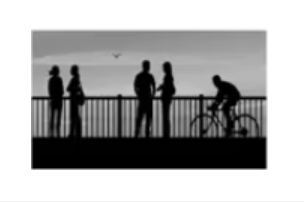
\includegraphics[width=12cm]{Image.png}
\end{figure}
}


\clearpage

 There are many vertical and horizontal edges in the image. The first thing to do is to detect these edges:
{
\begin{figure}[htp]
    \centering
    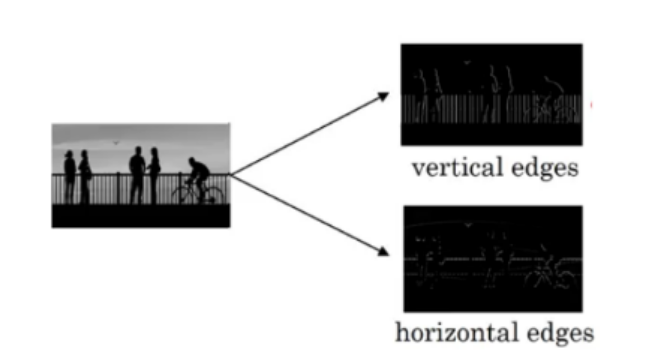
\includegraphics[width=500]{split.png}
\end{figure} }

But how do we detect these edges? To illustrate this, let’s take a 6 X 6 greyscale image (i.e. only one channel): 
% \clearpage
{
\begin{figure}[htp]
    \centering
    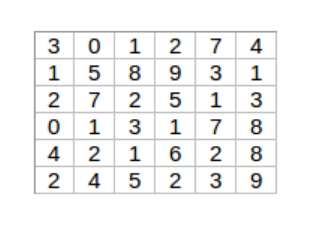
\includegraphics[width=5cm]{greyscale.png}
\end{figure}
}

Next, we convolve this 6 X 6 matrix with a 3 X 3 filter: 
{
\begin{figure}[htp]
    \centering
    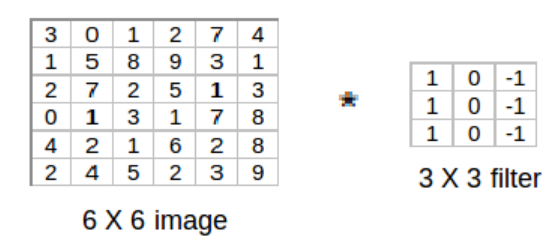
\includegraphics[width=250]{matrix.png}
\end{figure}
}

\clearpage

After the convolution, we will get a 4 X 4 image. The first element of the 4 X 4 matrix will be calculated as:

{
\begin{figure}[htp]
    \centering
    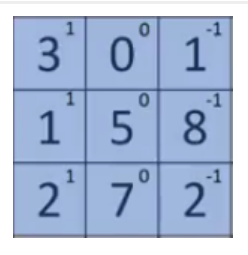
\includegraphics[width=5cm]{3x3_matrix.png}
\end{figure}
}

So, we take the first 3 X 3 matrix from the 6 X 6 image and multiply it with the filter. Now, the first element of the 4 X 4 output will be the sum of the element-wise product of these values, i.e. 3*1 + 0 + 1*-1 + 1*1 + 5*0 + 8*-1 + 2*1 + 7*0 + 2*-1 = -5. To calculate the second element of the 4 X 4 output, we will shift our filter one step towards the right and again get the sum of the element-wise product:

{
\begin{figure}[htp]
    \centering
    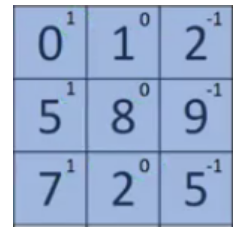
\includegraphics[width=5cm]{F_3x3_matrix.png}
\end{figure}
}

Similarly, we will convolve over the entire image and get a 4 X 4 output: 
{
\begin{figure}[htp]
    \centering
    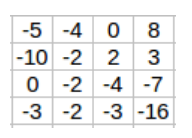
\includegraphics{f1_m.png}
\end{figure}
}


\clearpage

So, convolving a 6 X 6 input with a 3 X 3 filter gave us an output of 4 X 4. Consider one more example: 

{
\begin{figure}[htp]
    \centering
    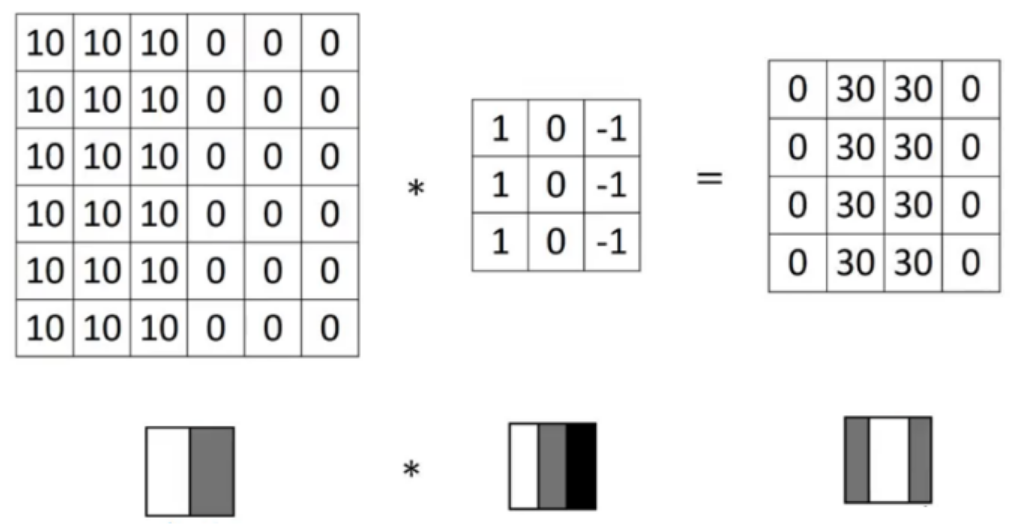
\includegraphics[width=300]{Final_output.png}
\end{figure}
}
Note: Higher pixel values represent the brighter portion of the image and the lower pixel values represent the darker portions. This is how we can detect a vertical edge in an image.

\textbf{MORE ON EDGE DETECTION}

The type of filter that we choose helps to detect the vertical or horizontal edges. We can use the following filters to detect different edges: 

{
\begin{figure}[htp]
    \centering
    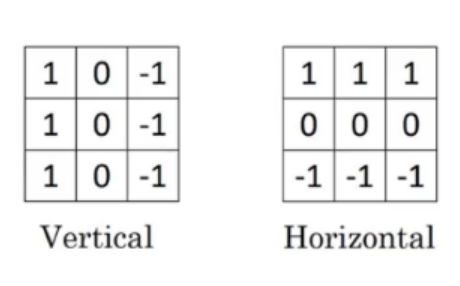
\includegraphics[width=8cm]{V_H_matrix.png}
\end{figure}
}

Some of the commonly used filters are: 

{
\begin{figure}[htp]
    \centering
    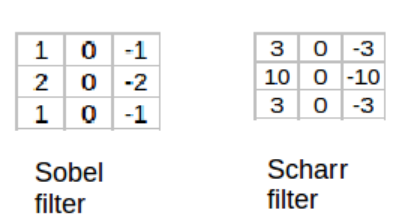
\includegraphics[width=8cm]{filter.png}
\end{figure}
}

The Sobel filter puts a little bit more weight on the central pixels. Instead of using these filters, we can create our own as well and treat them as a parameter which the model will learn using backpropagation. 
\clearpage

\textbf{PADDING :}

We have seen that convolving an input of 6 X 6 dimension with a 3 X 3 filter results in 4 X 4 output. We can generalize it and say that if the input is n X n and the filter size is f X f, then the output size will be (n-f+1) X (n-f+1):

    Input: n X n
    Filter size: f X f
    Output: (n-f+1) X (n-f+1)
    
There are primarily two disadvantages here:

    Every time we apply a convolutional operation, the size of the image shrinks
    Pixels present in the corner of the image are used only a few number of times during convolution as compared to the central pixels. Hence, we do not focus too much on the corners since that can lead to information loss

To overcome these issues, we can pad the image with an additional border, i.e., we add one pixel all around the edges. This means that the input will be an 8 X 8 matrix (instead of a 6 X 6 matrix). Applying convolution of 3 X 3 on it will result in a 6 X 6 matrix which is the original shape of the image. This is where padding comes to the fore: 

   -Input: n X n
    -Padding: p
    -Filter size: f X f
    -Output: (n+2p-f+1) X (n+2p-f+1)

There are two common choices for padding:

    1)Valid: It means no padding. If we are using valid padding, the output will be (n-f+1) X (n-f+1)
    
    2)Same: Here, we apply padding so that the output size is the same as the input size, i.e.,
    n+2p-f+1 = n
    So, p = (f-1)/2
    
    
    
  
 \textbf{ STRIDED CONVOLUTIONS :}
  
  Suppose we choose a stride of 2. So, while convoluting through the image, we will take two steps – both in the horizontal and vertical directions separately. The dimensions for stride s will be: 
 
    -Input: n X n
    
    -Padding: p
    
    -Stride: s
    
    -Filter size: f X f
    
    -Output: [(n+2p-f)/s+1] X [(n+2p-f)/s+1]

Stride helps to reduce the size of the image, a particularly useful feature. 

\clearpage


\textbf{CONVOLUTIONS OVER VOLUME :}

Suppose, instead of a 2-D image, we have a 3-D input image of shape 6 X 6 X 3. How will we apply convolution on this image? We will use a 3 X 3 X 3 filter instead of a 3 X 3 filter. Let’s look at an example:

    -Input: 6 X 6 X 3
    
    -Filter: 3 X 3 X 3

The dimensions above represent the height, width and channels in the input and filter. Keep in mind that the number of channels in the input and filter should be same. This will result in an output of 4 X 4. Let’s understand it visually: 

{
\begin{figure}[htp]
    \centering
    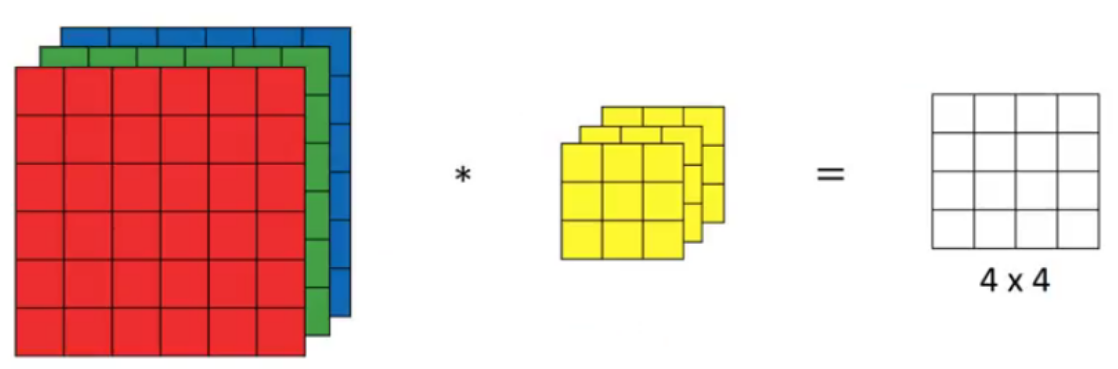
\includegraphics[width=10cm]{C_Volume.png}
\end{figure}
}

Since there are three channels in the input, the filter will consequently also have three channels. After convolution, the output shape is a 4 X 4 matrix. So, the first element of the output is the sum of the element-wise product of the first 27 values from the input (9 values from each channel) and the 27 values from the filter. After that we convolve over the entire image. 

Instead of using just a single filter, we can use multiple filters as well. How do we do that? Let’s say the first filter will detect vertical edges and the second filter will detect horizontal edges from the image. If we use multiple filters, the output dimension will change. So, instead of having a 4 X 4 output as in the above example, we would have a 4 X 4 X 2 output (if we have used 2 filters): 

{
\begin{figure}[htp]
    \centering
    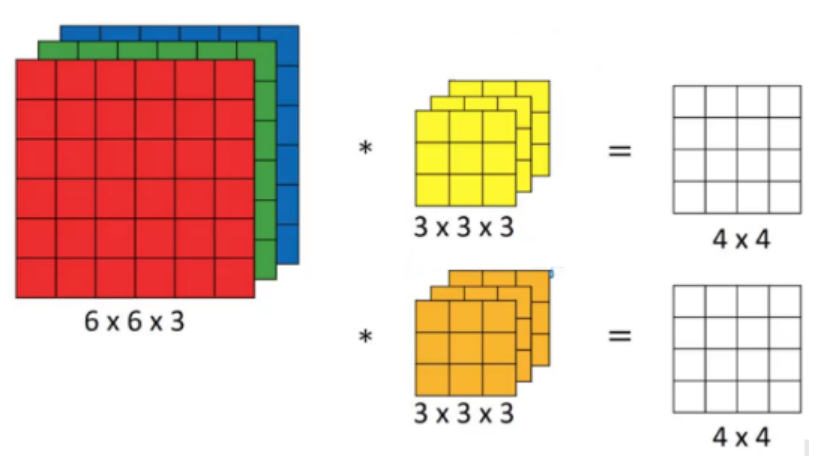
\includegraphics[width=10cm]{F_Volume.png}
\end{figure}
}

\textbf{Generalized dimensions can be given as:}

    -Input: n X n X nc
    
    -Filter: f X f X nc
    
    -Padding: p
    
    -Stride: s
    
    -Output: [(n+2p-f)/s+1] X [(n+2p-f)/s+1] X nc’

Here, nc is the number of channels in the input and filter, while nc’ is the number of filters. 


\textbf{ONE LAYER OF A CONVOLUTIONAL NETWORK:}

Once we get an output after convolving over the entire image using a filter, we add a bias term to those outputs and finally apply an activation function to generate activations. This is one layer of a convolutional network. Recall that the equation for one forward pass is given by: 
z[1] = w[1]*a[0] + b[1]

a[1] = g(z[1]) 

In our case, input (6 X 6 X 3) is a[0]and filters (3 X 3 X 3) are the weights w[1]. These activations from layer 1 act as the input for layer 2, and so on. Clearly, the number of parameters in case of convolutional neural networks is independent of the size of the image. It essentially depends on the filter size. Suppose we have 10 filters, each of shape 3 X 3 X 3. What will be the number of parameters in that layer? Let’s try to solve this: 

 Number of parameters for each filter = 3*3*3 = 27
There will be a bias term for each filter, so total parameters per filter = 28
As there are 10 filters, the total parameters for that layer = 28*10 = 280

No matter how big the image is, the parameters only depend on the filter size. Awesome, isn’t it? Let’s have a look at the summary of notations for a convolution layer: 

    -f[l] = filter size
    
    -p[l] = padding
    
    -s[l] = stride
    
    -n[c][l] = number of filters
    
    Let’s combine all the concepts we have learned so far and look at a convolutional network example. 
       
\textbf{SIMPLE CONVOLUTIONAL NETWORK EXAMPLE:}
      
{
\begin{figure}[htp]
    \centering
    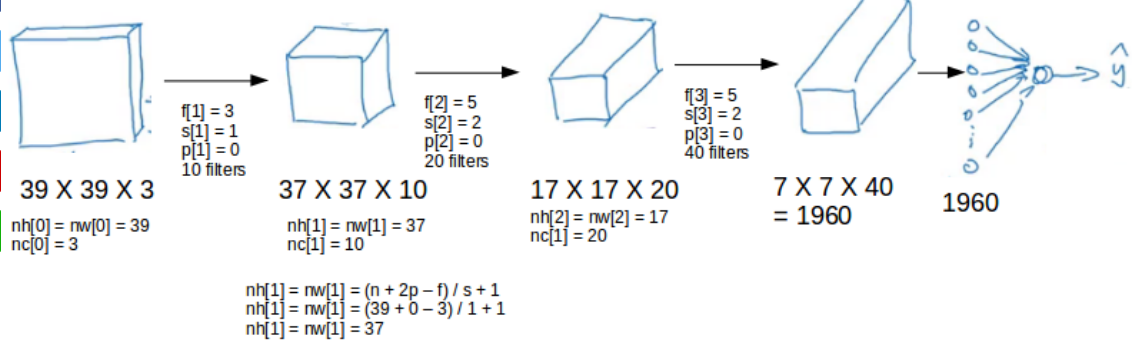
\includegraphics[width=15cm]{CNN.png}
\end{figure}
}

We take an input image (size = 39 X 39 X 3 in our case), convolve it with 10 filters of size 3 X 3, and take the stride as 1 and no padding. This will give us an output of 37 X 37 X 10. We convolve this output further and get an output of 7 X 7 X 40 as shown above. Finally, we take all these numbers (7 X 7 X 40 = 1960), unroll them into a large vector, and pass them to a classifier that will make predictions. This is a microcosm of how a convolutional network works.

\clearpage

There are a number of hyperparameters that we can tweak while building a convolutional network. These include the number of filters, size of filters, stride to be used, padding, etc. We will look at each of these in detail later in this article. Just keep in mind that as we go deeper into the network, the size of the image shrinks whereas the number of channels usually increases. 

\textbf{In a convolutional network (ConvNet), there are basically three types of layers:}

    \textbf{1)Convolution layer}
    
   \textbf{2) Pooling layer}
    
    \textbf{3)Fully connected layer}
    
    
\textbf{POOLING LAYERS:}

Pooling layers are generally used to reduce the size of the inputs and hence speed up the computation. Consider a 4 X 4 matrix as shown below: 

{
\begin{figure}[htp]
    \centering
    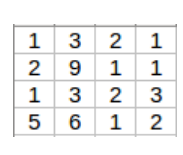
\includegraphics[]{matrix1.png}
\end{figure}
}

Applying max pooling on this matrix will result in a 2 X 2 output: 

{
\begin{figure}[htp]
    \centering
    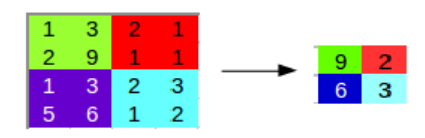
\includegraphics[width=10cm]{pooling.png}
\end{figure}
}

For every consecutive 2 X 2 block, we take the max number. Here, we have applied a filter of size 2 and a stride of 2. These are the hyperparameters for the pooling layer. Apart from max pooling, we can also apply average pooling where, instead of taking the max of the numbers, we take their average. In summary, the hyperparameters for a pooling layer are: 

    1)Filter size
    
    2)Stride
    
    3)Max or average pooling

If the input of the pooling layer is nh X nw X nc, then the output will be [{(nh – f) / s + 1} X {(nw – f) / s + 1} X nc]

\clearpage

\textbf{CNN EXAMPLE:} 

{
\begin{figure}[htp]
    \centering
    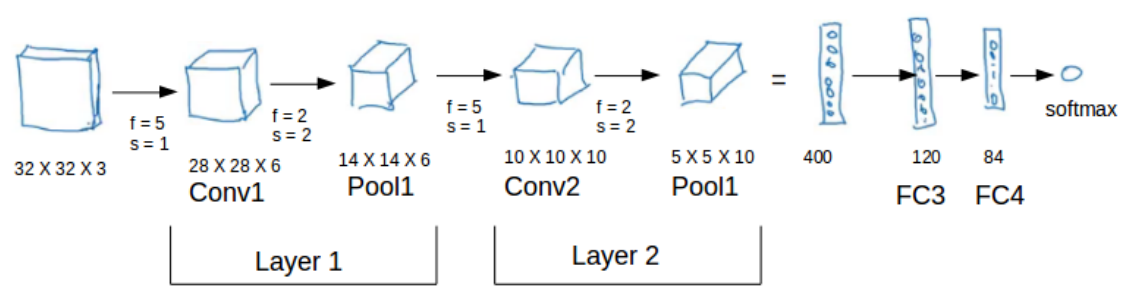
\includegraphics[width=15cm]{CNN_eg.png}
\end{figure}
}

\textbf{CLASSIC  NETWORKS :} 

\textbf{LeNet-5}
{
\begin{figure}[htp]
    \centering
    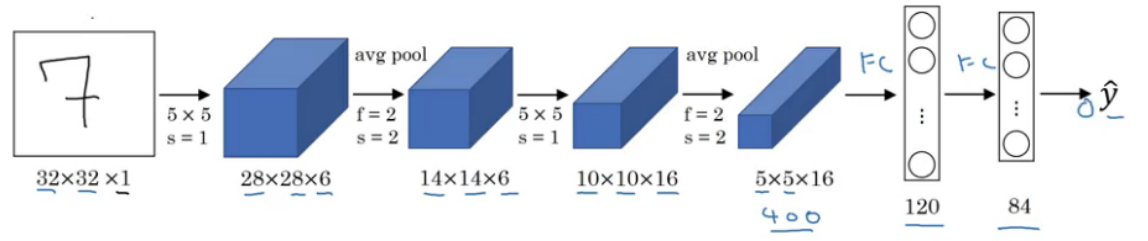
\includegraphics[width=15cm]{LeNet5.png}
\end{figure}
}

It takes a grayscale image as input. Once we pass it through a combination of convolution and pooling layers, the output will be passed through fully connected layers and classified into corresponding classes. The total number of parameters in LeNet-5 are: 

    -Parameters: 60k
    
    -Layers flow: Conv - Pool - Conv - Pool - FC - FC - Output
    
    -Activation functions: Sigmoid/tanh and ReLu
    
\textbf{ AlexNet  } 

{
\begin{figure}[htp]
    \centering
    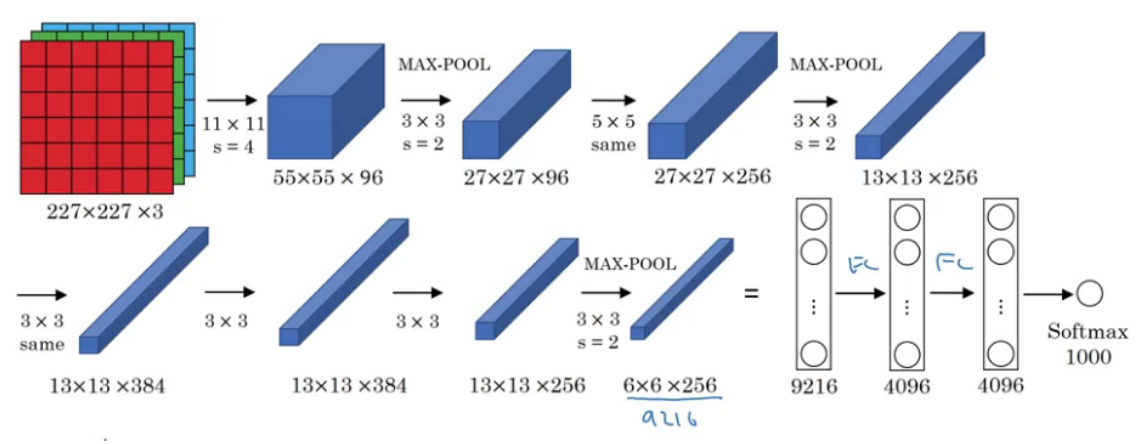
\includegraphics[width=15cm]{AlexNet.png}
\end{figure}
}

This network is similar to LeNet-5 with just more convolution and pooling layers:

    -Parameters: 60 million
    -Activation function: ReLu
    
\clearpage  

\textbf{VGG-16  }  

The underlying idea behind VGG-16 was to use a much simpler network where the focus is on having convolution layers that have 3 X 3 filters with a stride of 1 (and always using the same padding). The max pool layer is used after each convolution layer with a filter size of 2 and a stride of 2. Let’s look at the architecture of VGG-16: 

{\begin{figure}[htp]
    \centering
    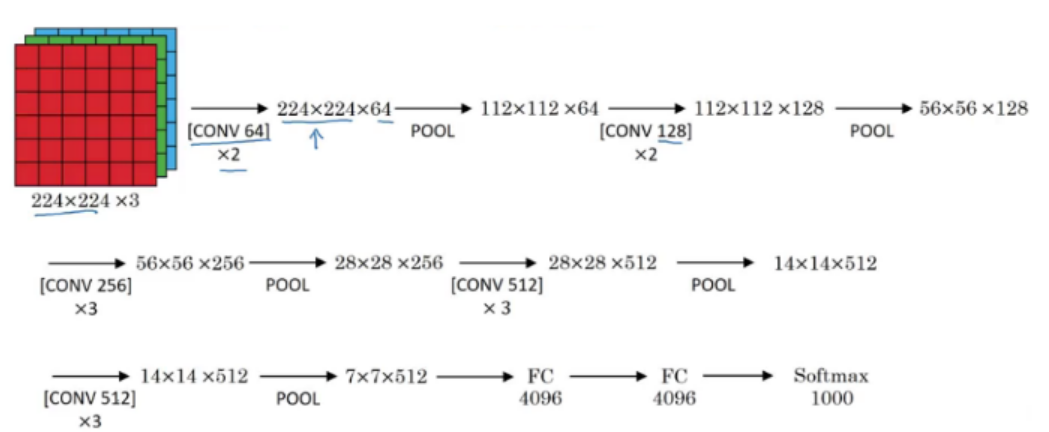
\includegraphics[width=15cm]{VGG-16.png}
\end{figure}}

As it is a bigger network, the number of parameters are also more.

   -Parameters: 138 million



\textbf{Summary:}

 We have covered the big picture of CNN and couple of underlying architectures and techniques. This report would work as the building block for foundation and introduction for CNN.


\end{document}